\section{需求分析}
   需求中要求程序求出n, x, y的关系,使加里森成为最后一个队员。所以我们可以设计一个
程序,利用它来求出一定范围内所有三元组(n, x, y)满足1号队员最后一个执行任务。
由于确定了n与y后,x是唯一的,所以我们可以设置上界$N_{max}$与$Y_max$,输出所有符合
$1 \leqslant n \leqslant  N_{max}$ 与 $1 \leqslant y \leqslant  Y_{max}$的三元组。


这样,我们的输入仅有一行,为$N_{max}$与$Y_{max}$。
同时,我们对输入作出要求,$N_{max} \geqslant 1$ 且 $Y_{max} \geqslant 1$
然后我们会按顺序输出$(n, y, x)$,每个占一行,先从$n = 1$开始输出到$n = N_{max}$,才能递增$y$。

例如输入

   2 2


输出为
\begin{enumerate}
   \item (1, 1, 1)
   \item (2, 1, 1)
   \item (1, 2, 1)
   \item (2, 2, 2)
\end{enumerate}


同时如果输入非法,例如 -1 2


输出为


输入错误(Input Error)

\section{概要设计}
在link.h中定义链表数据结构:
\begin{enumerate}
   \item 每一个link对象都保存一个head指针,指向链表的表头。
   \item solve函数为链表对象唯一对外可以操作的函数,返回特定$n$,$y$下的$x$;
   \item delete\_node函数删去链表结点的下一个结点;
   \item insert使用头插插入一个新的结点;
\end{enumerate}


main.cpp:
\begin{enumerate}
   \item 调用link的solve得到特定$n$与$y$的结果。
\end{enumerate}

\section{详细设计}


\begin{figure}[H]
   \centering
   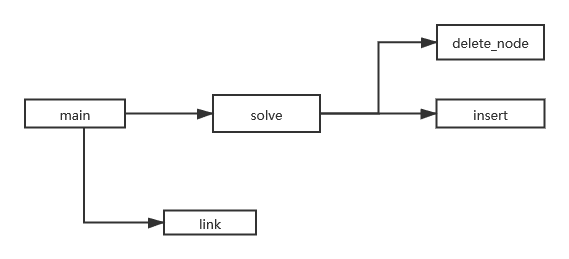
\includegraphics[width=0.5\textwidth]{images/process.png}
   \caption{总体流程图}
\end{figure}


\begin{algorithm}[htb] 
\caption{ Solve } 
\label{alg:Framwork} 
\begin{algorithmic}[1]
\Require
队员总数n与间隔y
\Ensure
加里森的位置
\State 初始化链表,用链表模拟队员的顺序
\State 用$cur$指针指向头指针
\While {$cur$不是最后一个队员} 
\State $cur$向后移动$y-1$次
\State 删除$cur$指向的下一个队员
\EndWhile
\State 利用最后一个队员的编号计算$x$的值 \\
\Return $x$; 
\end{algorithmic} 
\end{algorithm}

\begin{algorithm}[htb] 
   \caption{ insert } 
   \label{alg:Framwork} 
   \begin{algorithmic}[1]
   \Require
   队员的编号
   \State 初始化结点,结点的编号为队员的编号
   \State 结点的后驱指向head的后驱
   \State head的后驱指向结点
   \end{algorithmic} 
   \end{algorithm}

   \begin{algorithm}[htb] 
\caption{ delete\_node } 
\label{alg:Framwork} 
\begin{algorithmic}[1]
\Require
前驱结点pre
\Ensure
删除结点的后驱
\State pre的后驱设置为要删除结点的后驱
\State 释放原pre的后驱
\end{algorithmic} 
\end{algorithm}


\section{调试分析报告}
   在代码编写过程中,笔者曾经遇到过使用delete\_node函数删除过头指针的情况。
   这是因为当$cur$指向最后一名队员时,没有直接过渡到头指针造成的。


   对于这个过程的算法分析较为简单,我们模拟一组$(n, x, y)$操作的复杂度为$O(ny)$,因为我们每$y$个人删去一个人,总共要删去$n$个人。
   随后我们计算所有情况下的计算次数$$ \sum^{Y_{max}}_{y = 1}{\sum^{N_{max}}_{n = 1}{ny}} = O(N_{max}^2Y_{max}^2)$$

   同时,在分析固定$y$情况下的结果时,我们得到了一些有趣的关系图片。
   在固定$y$且$x = 1$的情况下,设$result_n$为在此情况下最后出界的队员编号。
   在已知$result$的情况下,我们可以反推出在何种情况下可以使加里森成为最后一个队员。

   \begin{figure}[H]
      \centering
      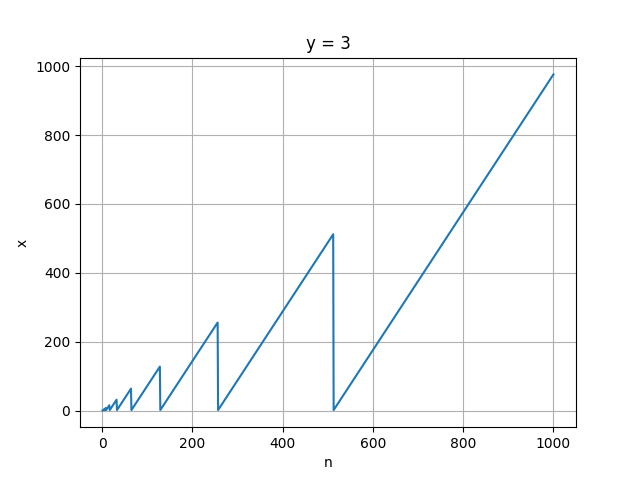
\includegraphics[width=0.5\textwidth]{images/y3.png}
      \caption{y = 3时n与x的关系}
   \end{figure}


   \begin{figure}[H]
      \centering
      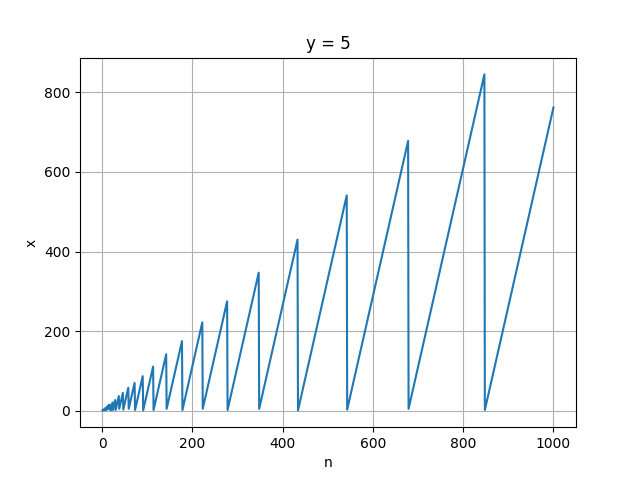
\includegraphics[width=0.5\textwidth]{images/y5.png}
      \caption{y = 5时n与x的关系}
   \end{figure}


   我们惊奇的发现在固定y的情况下,n与x的关系是一个前后之差为y的等差数列,并且有一定的周期性。
   根据多次测试后,我们得出了一个可靠的规律。
   $$ result_{n} = (result_{n-1} + y - 1) \% n + 1 $$

   利用这个关系,我们可以不使用模拟,而使用递推的方式得出结果,递推算法的复杂度为$O(N_{max}Y_{max})$

\section{用户使用说明}

   用户可以使用IDE或者手动编译源代码Joseph.cpp,获得可执行文件。
   
   笔者使用的gcc版本为8.1.0
   运行可执行文件后,按照规定的格式输入数值。
   程序返回的结果会重定向到当前文件夹下的output.out.

\section{测试结果}

   测试数据保存在test.in中,而测试的正确结果保存在test.out中。
   这里的test.out经手工计算获得,用于测试程序的正确性。
   代码中设定了测试相关的宏,在定义TEST的情况下,编译的程序会直接从test.in中读入数据


   接下来对所有测试结果进行说明:
   \begin{enumerate}
      \item $(1,1,1)$  只有一个人
      \item $(2,1,2)$  2(x)
      \item $(3,1,2)$  2(x) -> 3(x)
      \item $(1,2,1)$  只有一个人
      \item $(2,2,1)$  1->2(x)
      \item $(3,2,2)$  2->3(x)->1->2(x)
      \item $(1,3,1)$  只有一个人
      \item $(2,3,2)$  2->1->2(x)
      \item $(3,3,3)$  3->1->2(x)->3->1->3(x)
   \end{enumerate}

   再使用fc output.out test.out比较程序输出的结果。


